% Block Diagram of Power System Stabilizer (PSS) in TikZ
% latexdraw.com
% 08/02/2021 at 07:42

\documentclass[border=0.2cm]{standalone}

% Required packages and libraries
\usepackage{tikz,amsmath}

\usetikzlibrary{shapes.geometric,positioning}

\begin{document}

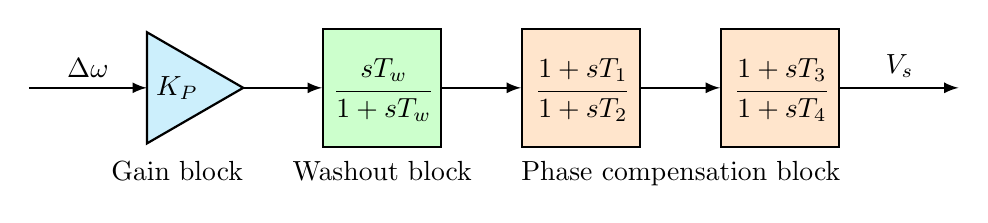
\begin{tikzpicture}[thick,
	gain/.style = {
		draw, 
		isosceles triangle,
		isosceles triangle apex angle=60,
		minimum height = 2em,
		outer sep=0},
	TFblock/.style= {
		draw,  
		minimum size=1.5cm}]

% Gain block
\node [gain,fill=cyan!20] (a) {$K_P$};

% Washout Filter Block
\node [TFblock,fill=green!20,] (b) [right= of a] {$\cfrac{sT_{w}}{1+sT_w}$};

% Phase Compensation Block
\node [TFblock,fill=orange!20] (c) [right =of b] {$\cfrac{1+sT_{1}}{1+sT_2}$};
\node [TFblock,fill=orange!20] (d)[right =of c] {$\cfrac{1+sT_{3}}{1+sT_4}$};

% Arrows
\draw[-latex] (a.west)++(-1.5,0) edge node[above] {$\Delta \omega$} (a.west)
	(a.east) edge (b.west)
	(b.east) edge (c.west)
	(c.east) edge (d.west)
	(d.east) -- node[above] {$V_s$} ++(1.5,0) ;

% Labels
\node[below=0.8cm] at (a){ Gain block};
\node[below=0.8cm] at (b){ Washout block};
\node[below=0.8cm] at (barycentric cs:c=1,d=1){ Phase compensation block};

\end{tikzpicture}

\end{document}